%!TEX root = main.tex

\chapter{Theory}
\section{Starcraft}

\begin{figure}[h!tb]
\centering
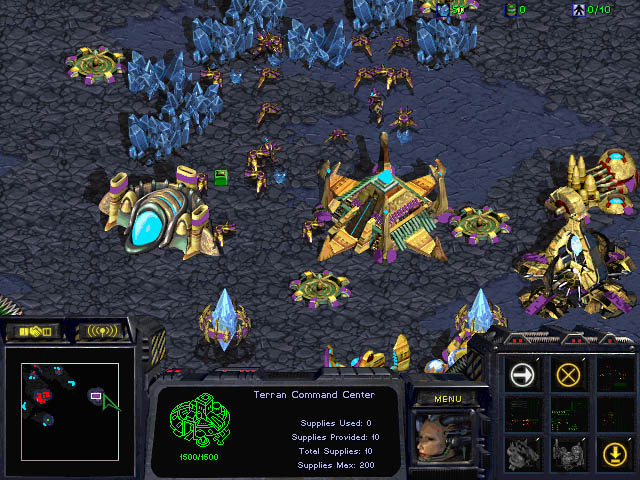
\includegraphics[scale=0.5]{graphics/scbw.jpg}
\caption{Star Craft Brood War}
\label{fig:scbwIntro}
\end{figure}
StarCraft is on the surface a very simple game, it has only three different playable races, a
handful of different buildings and units, and relatively simple to comprehend
goals. But once you start analyzing the game, the reality is quite different. The brood war expansion pack was released back in 1998, and has been played at a high level since that and all the way up to today. And the meta game has evolved during the entire lifespan of the game and is still changing today with new tactics showing up from tournament to tournament.
\cite{blizzardstarcraft}

When playing at a really high level you are working with really small windows of opportunity, often called timings. And it is these timings that enable a game with what should in theory be simple elements to have such complex and evolving strategies.

\subsection{Terran}
Terran are the human faction of StarCraft, a futuristic version of man today. They are known for high adaptability with a good variety of defensive and mobile armies. They are best known for their mobile biological armies, or their slow moving turtling tech(tanks) armies that slowly creeps across the map and secures section for section. This versatility makes them a great class with a lot of different possible strategies and combinations that can be effective. 
\\
\textit{
Strengths: \\
Mobility, great defense, build anywhere, cloaking, versatility, Marines, strong through whole tech-tree, easy to learn, instant cloak detection, ability to repair buildings and most units. \\
Weaknesses: \\
Tendency to "turtle", need lots of space, require active scouting, require micromanagement for special abilities, vulnerable to Dark Swarm, buildings burn up when highly damaged. 
} 
\cite{terranoverview}
\\

The Terran worker is the Space Construction Vehicle (SCV). This unit can gather minerals, build buildings and unique for the Terran race repair other mechanical units or buildings. When constructing buildings the unit has to \textit{build} the building from the initial placement to the building is complete, meaning it will be unable to perform other action in this time, unless the construction is halted. Like mentioned before it can also repair mechanical units like tanks if they have taken damage, but to perform this action they have to be pulled from other tasks like mining minerals so it is a two edged sword. 

Terran buildings also have a unique feature in that they can lift of the ground and fly around after being constructed. They can then land in a new location and continue production of units or upgrades. Some buildings can also create add-ons that unlocks new units and upgrades for that building. Terran also have a unique building in the bunker. This a a defensive building where  biological units can seek refuge and fire from them.  While being useless on it's own, the building can be a death trap when filled with infantry. The bunker can also be repaired by an SCV like any other building so take out the SCVs are priority if you are trying to get a bunker down. 

\section{Artificial Intelligences for StarCraft}
There have been a handful of relatively successful AIs for StarCraft.

\subsection{In-game AI}
The in-game AI is considered not very good.

\subsection{Berkeley Overmind}
This is considered one of the best AIs, not perhaps because it is very complex,
but because it has a solid ``cheese'' and has been well-tweaked.


\section{Architectures}
\subsection{General architectures}
\subsubsection{}
\subsection{Cognitive Architectures}
\paragraph{Global Workspace Theory}
\paragraph{Cognitive Models in game AIs}
\cite{Arrabales2009}
